\documentclass{article}
\usepackage[utf8]{inputenc}
\usepackage{listings} 
\usepackage[english,russian]{babel} 
\usepackage[a4paper,top=3cm,bottom=2cm,left=1.75cm,right=1.75cm,marginparwidth=1.75cm]{geometry}
\usepackage{amssymb}
\usepackage{esint}
\usepackage{amsmath,amsthm,amssymb}
\usepackage{indentfirst}
\usepackage{hyperref}
\usepackage{csquotes}
\usepackage{minted}
\usepackage{graphicx}
\usepackage{caption}

\theoremstyle{plain}
\newtheorem{theorem}{Теорема}[section]

\theoremstyle{plain}
\newtheorem{consequence}[theorem]{Следствие}

\theoremstyle{plain}
\newtheorem{lemma}{Лемма}[section]

\theoremstyle{plain}
\newtheorem{claim}{Утверждение}[section]

\theoremstyle{definition}
\newtheorem{definition}{Определение}[section]

\theoremstyle{remark}
\newtheorem{remark}{Замечание}[section]

\title{Построение модели акционерной страховой компании в рамках модели риска Крамера-Лундберга}
\author{Климовицкий Роман}

\begin{document}

\maketitle

\large

\section{Введение}

Наиболее распространенными и хорошо описанными моделями страхования являются модели страхования Крамера-Лундберга и Спарре-Андерсена:

\begin{itemize}
    \item \textbf{Модель страхования Крамера-Лундберга} \\
    В данной модели капитал страховой компании определяется как случайный процесс $\{Y_t, t \geq 0\}$ следующим образом:

    \begin{equation}
    \label{Kramer-Lundberg}
        Y_t = y_0 + ct - \displaystyle \sum_{k = 1}^{N_t} \eta_k,
    \end{equation}
    
    где $y_0, c > 0$, $N_t$ -- пуассоновский процесс интенсивности $\lambda$, $\{\eta_k\}_{k = 1}^{\infty}$ -- независимые одинаково распределенные случайные величины. В данной модели в качестве параметра $y_0$ берется начальный капитал компании, $c$ -- скорость получения премий (например, от застрахованных лиц), процесс $N_t$ определяет моменты наступления страховых случаев, а $\eta_k$ -- размеры страховых выплат по ним. Подобная модель страхования может успешно применятся для моделирования капитала компании, занимающейся страхованием имущества или страхованием от несчастных случаев.

    \item \textbf{Модель страхования Спарре-Андерсена} \cite{Sparre-Andersen} является обобщением модели Крамера-Лундберга: капитал страховой компании определяется аналогичным образом, но случайный процесс $N_t$, согласно которому определяются моменты выплат, считается произвольным процессом восстановления:
    
    \begin{equation}
    \label{Sparre-Andersen}
        X_t = x + ct - \displaystyle \sum_{i = 1}^{N_t} \xi_i,
    \end{equation}
    
    где $x, c > 0$, $N_t$ -- процесс восстановления, $\{\xi_i\}_{i = 1}^{\infty}$ -- независимые одинаково распределенные случайные величины.
\end{itemize}
 

Далее проведем краткий обзор результатов, полученных в ходе работ с данными моделями или их разновидностями.
    
\section{Обзор литературы}

В книге Булинского А. В. и Ширяева А. Н. \cite{Shiryaev_stochastic} рассмотрен классический случай модели страхования Крамера-Лундберга и получен фундаментальный результат для оценки вероятности разорения. Доказательство полученной оценки проведено с помощью мартингальных методов, а именно -- при помощи теоремы об остановке для мартингалов. % Желательно здесь добавить ссылку на актуальную работу. Предложение актуально. 

Бойков А.В. в своей работе \cite{KL_premium} рассматривает модель Крамера-Лундберга, в которой поступления в капитал страховой компании поступают дискретно в соответствии с отдельным пуассоновским процессом. По аналогии с классической моделью Крамера-Лундберга, для вероятностей неразорения получены интегральные уравнения и экспоненциальные оценки.

Необычную модификацию модели Спарре-Андерсена в своей работе \cite{SA_dividends} изучает Муромская А.А. Пусть страховая компания, для которой строится модель, является акционерным обществом и платит дивиденды в соответствии с линейной барьерной стратегией: при превышении капитала $U_t = Y_t - D_t$ ($D_t$ -- сумма дивидендов, выплаченная компанией к моменту времени $t$) барьерной функции $b_t$ поступающая премия начинает полностью или частично выплачиваться в качестве дивидендов. В случае, когда $b_t = b + at$ является линейной, можно считать, что до следующего страхового случая интенсивность выплаты дивидендов равна $c - a$. Таким образом, капитал компании сохраняется на уровне $b_t$ до очередной страховой выплаты.

За основу в дальнейшей работе возьмем именно модель страховой компании, являющейся акционерным обществом, поскольку данная проблема до конца не изучена, что открывает дополнительные возможности для экспериментов.
%Желательно добавить структуру дальнейшей работы.

\section{Постановка задачи}
\label{Problem_Description}

Для упрощения задачи в качестве базовой модели возьмем модель страхования Крамера-Лундберга (\ref{Kramer-Lundberg}).

Пусть $D_t$ -- сумма выплаченных дивидендов к моменту времени $t$. Тогда результирующий капитал компании в момент времени $t$ равен $U_t = Y_t - D_t$.

Как уже было упомянуто, рассматривается некоторая барьерная функция $b_t$, определяющая нижнюю грань капитала компании для выплаты дивидендов:

\begin{enumerate}
    \item Если $U_t < b_t$, дивиденды не выплачиваются;
    \item Если $U_t > b_t$, в момент времени $t$ единовременно выплачиваются дивиденды в размере $U_t - b_t$ (такое может быть только при $t = 0$, поэтому без ограничения общности можно считать, что всегда выполнено $U_t \leq b_t$);
    \item После наступления момента $U_t = b_t$ значение капитала остается на уровне $b_t$ до наступления следующего страхового случая или до превышения барьерной функцией капитала.
\end{enumerate}

В дальнейшей работе попробуем получить оценку вероятности разорения компании в случае линейной барьерной стратегии аналогично стандартной модели Крамера-Лундберга: когда $b_t = b + at$, в том числе оценку вероятности разорения на интервале. Также смоделируем описанный процесс на одном из языков программирования с возможностью задания произвольной барьерной функции.


\section{Теоретическая часть}

\subsection{Оценка вероятности разоерния в модели Крамера-Лундберга}
\label{KL_Shiryaev_section}

Перед тем, как приступить к рассмотрению модификации модели Крамера-Лундберга, рассмотрим метод нахождения оценки вероятности разорения для его стандартного варианта (\ref{Kramer-Lundberg}). Кратко осветим основные моменты из работы Ширяева, Булинского \cite{Shiryaev_stochastic}.

Для начала предположим, что

\begin{equation}
    \psi(v) = \mathbb{E} e^{v \eta_1} < \infty,\ v > 0.
\end{equation}

Как правило, выплаты $\eta_k$ ограничены, поэтому такое предположение вполне реалистино. Далее, воспользовавшись формулой полной вероятности и свойствами пуассоновского процесса, можем получить:

\begin{equation}
\label{KL_inter_0}
    \mathbb{E} e^{-v(Y_t - Y_s)} = e^{(t - s)g(v)}, \text{ где } g(v) = \lambda(\psi(v) - 1) - vc.
\end{equation}

Подставляя в (\ref{KL_inter_0}) $Y_0 = y_0$, получаем:

\begin{equation}
\label{KL_inter_1}
    0 < \mathbb{E} e^{-v Y_t} = e^{t g(v) - v y_0} < + \infty,\ t \in \mathbb{R}_+.
\end{equation}


Введем процесс $Z_t$:

\begin{equation}
    Z_t = e^{-v Y_t - g(v) t}
\end{equation}

и покажем, что он является мартингалом относительно естественной фильтрации $\mathbb{F}^Y$ процесса $Y_t$. Понятно, что он будет согласован c $\mathbb{F}^Y$ -- $Z_t$ явно выражается через $Y_t$. То, что $Z_t$ является $L_1$-процессом, мы показали ранее (\ref{KL_inter_1}). Осталось посчитать условное математическое ожидание при $t > s$:

\begin{equation}
\begin{aligned}
    \mathbb{E} (Z_t | \mathcal{F}_s^Y) = \mathbb{E} (e^{-v Y_t - g(v) t} | \mathcal{F}_s^Y) = \mathbb{E} (e^{-v (Y_t - Y_s) - v Y_s - g(v) t} | \mathcal{F}_s^Y) = \\
    \\ = e^{- v Y_s - g(v) t}\ \mathbb{E} (e^{-v (Y_t - Y_s)} | \mathcal{F}_s^Y) = e^{- v Y_s - g(v) t}\ \mathbb{E} (e^{-v (Y_t - Y_s)}) = \\
    = e^{- v Y_s - g(v) t} \cdot e^{(t - s)g(v)} = e^{-v Y_s - g(v) s} = Z_s.
\end{aligned}
\end{equation}

Далее вводим момент разорения:

\begin{equation}
    \tau = \inf \{ t > 0 : Y_t < 0 \}.
\end{equation}

По построению видно, что он является марковским моментом относительно фильтрации $\mathbb{F^Y}$. Для применения теоремы об остановке нам нужны ограниченные марковские моменты. Поэтому будем рассматривать момент $\min (\tau, t)$. Применим теорему об остановке для процесса $Z_t$ и данного марковского момента:

\begin{equation}
\begin{aligned}
    e^{-v y_0} = \mathbb{E} Z_0 = \mathbb{E} Z_{\min (\tau, t)} \geq \mathbb{E} e^{-v Y_{\min (\tau, t)} - g(v) \cdot \min (\tau, t)} \mathrm{I} (\tau \leq t) = \mathbb{E} e^{-v Y_\tau - g(v) \tau} \mathrm{I} (\tau \leq t) \geq \\
    \geq |\ Y_\tau \leq 0 \text{ п.н. в силу непр. траекторий}\ | \geq \mathbb{E} e^{-g(v) \tau} \mathrm{I} (\tau \leq t) \geq \displaystyle \inf_{0 \leq s \leq t} e^{-g(v)s} \cdot \mathrm{P}(\tau \leq t).
\end{aligned}
\end{equation}

Таким образом,

\begin{equation}
    \mathrm{P} (\tau \leq t) \leq e^{-v y_0} \sup_{0 \leq s \leq t} e^{g(v)s}.
\end{equation}

Изучив функцию $g(v)$, введенную в (\ref{KL_inter_0}), и предположив, что $c - \lambda \mathbb{E} \eta_1 > 0$ можно понять, что у уравнения $g(v) = 0$ существует единственный положительный корень $v_0,\ g(v_0) = 0$. Отсюда заключаем, что

\begin{equation}
\label{KLDefaultUpperEstimation}
    \mathrm{P} (\tau \leq t) \leq e^{-v_0 y_0}\ \forall t \in \mathbb{R}_+ \implies \mathrm{P} (\tau < \infty) \leq e^{-v_0 y_0}.
\end{equation}

\subsection{Модель Крамера-Лундберга со стохастическими премиями}

Без углубления в доказательство опишем аналогичный результат, полученный Бойковым А.В. для модели Крамера-Лундберга со стохастическими премиями \cite{KL_premium}.

Данная модель описывается следующим образом. Пусть у нас заданы два независимых пуассоновских процесса $N(t)$ и $N_1(t)$ с интенсивностями $\lambda$ и $\lambda_1$ соответственно, а также два набора случайных величин $\{ y_i \}_{i = 1}^{\infty}$ и $\{ c_i \}_{i = 1}^{\infty}$ с функциями распределения $F(u),\ F(0) = 0$ и $G(v),\ G(0) = 0$ -- так определяются размеры выплат по страховым случаям и размеры стохастических премий соотвественно, причем случайные величины в каждом из наборов распределены одинаково, все случайные величины независимы в совокупности, $x$ -- размер стартового капитала. Тогда под моделью Крамера-Лундберга со стохастическими премиями понимают процесс эволюцию капитала согласно процессу $X(t)$:

\begin{equation}
    X(t) = x + \displaystyle \sum_{i = 1}^{N_1(t)} c_i - \displaystyle \sum_{i = 1}^{N(t)} y_i.
\end{equation}


Данная модель более актуальна с точки зрения реального мира: доход страховой компании, как правило, не постоянен и зависит от множества факторов. Более того, доход обычно поступает не непрерывно, а так же, как и выплаты по страховым случаям -- частями.

Вероятность неразорения для стартового капитала $x$ определяется как $\varphi(x) = \mathrm{P}(X(t) \geq 0\ \forall t \in \mathbb{R}_+)$. В этом случае данная вероятность оценивается согласно теореме:

\begin{theorem}[\cite{KL_premium}, теорема 1]
    Вероятность неразорения $\varphi(x)$ удовлетворяет интегральному уравнению
    
    \begin{equation}
        (\lambda + \lambda_1) \varphi(x) = \lambda \displaystyle \int_0^x \varphi(x - u) dF(u) + \lambda_1 \displaystyle \int_0^{\infty} \varphi(x + v) dG(v).
    \end{equation}
    
    Если $R$ -- положительное решение характеристического уравнения
    
    \begin{equation}
        \lambda_1 (\mathbb{E} e^{-Rc_i} - 1) + \lambda (\mathbb{E} e^{-Ry_i} - 1) = 0,
    \end{equation}
    
    то $e^{-R(\Pi(t) - R(t)}$ -- мартингал и $\varphi(x) \geq 1 - e^{-Rx}$.
\end{theorem}


\subsection{Модель акционерной страховой компании в рамках модели Спарре-Андерсена}
\label{SA_dividents_subsection}

Муромская А.А. \cite{SA_dividends} рассматривает модель Спарре-Андерсена (\ref{Sparre-Andersen}) в связке с барьерной стратегией выплат дивидендов, описанной в разделе \ref{Problem_Description}. В качестве барьерной функциии берется линейная. На процесс $N_t$ накладываются дополнительные ограничения: интервалы между моментами выплат $\{ T_i \}$ имеют гамма-распределение с плотностью

\begin{equation}
    g(t) = \frac{\lambda^{\alpha}}{\Gamma(\alpha)} t^{\alpha - 1} e^{-\lambda t},\ t \geq 0,\ \alpha > 1,\ \lambda > 0.
\end{equation}

В процессе описания полученных результатов также рассматриваются характеристические уравнения ($G(t)$ -- функция распределения случайных величин $\{ T_i \}$):

\begin{equation}
\label{char_1}
    \displaystyle \int_0^{\infty} e^{ry} dF(y) \displaystyle \int_0^{\infty} e^{-crt} dG(t) = 1
\end{equation}

и

\begin{equation}
\label{char_2}
    \displaystyle \int_0^{\infty} e^{-qy} dF(y) \displaystyle \int_0^{\infty} e^{-t(Ra + qa - qc)} dG(t) = 1.
\end{equation}

Доказывается, что данные уравнения имеют единственные положительные корни -- $R$ и $Q$ соответственно. Тогда для вероятности разорения страховой компании $\varphi(x, b)$ в зависимости от начального капитала $x$ и барьерной функции $b_t = b + at$ можно выписать оценку:

\begin{equation}
\label{SA_div_proba}
    \psi(x, b) \leq e^{-Rx} + K e^{-(R + Q)b} e^{Qx},
\end{equation}

где

\begin{equation}
\label{K_equation}
    K = \frac{2^{\alpha - 1} (\lambda + Rc)^{\alpha - 1} R}{(\lambda + Ra + Qa - Qc)^{\alpha - 1} Q} + \frac{2^{\alpha - 1} \Big( (\lambda + Rc)^{\alpha} - (\lambda + Ra)^\alpha \Big)}{(\lambda + Ra)^\alpha - (\lambda + Ra + Qa - Qc)^\alpha}.
\end{equation}

\subsection{Модель акционерной страховой компании в рамках модели Крамера-Лундберга}

Теперь перейдем к задаче, поставленной в разделе \ref{Problem_Description}. Заметим, что времена между моментами скачков пуассоновского процесса интенсивности $\lambda$ имеют экспоненциальное распределение с параметром $\lambda$. Экспоненциальное распределение в свою очередь является частным случаем гамма-распределения: $\mathrm{Exp}(\lambda) \equiv \Gamma(1, 1 / \lambda)$. Это означает, что наша модель сводится к модели, рассмотренной Муромской А.А. в своей работе \cite{SA_dividends} и можем применить результат, описанный в подразделе \ref{SA_dividents_subsection}.

Выпишем уравнение, аналогичное (\ref{char_1}):

\begin{equation}
\begin{aligned}
\label{R_equation}
    \mathbb{E} e^{r \eta_1} \cdot \mathbb{E} e^{- cr T_1} = 1 \\
    \mathbb{E} e^{r \eta_1} = \Big( \mathbb{E} e^{-crT_1} \Big)^{-1} = \frac{cr + \lambda}{\lambda}.
\end{aligned}
\end{equation}

В действительности мы уже работали с подобным уравнением в подразделе \ref{KL_Shiryaev_section}, когда изучали поведение функции $g(v)$ из (\ref{KL_inter_0}). Там мы сослались на работу Ширяева А.Н. \cite{Shiryaev_stochastic}, где он показывает, что это уравнение имеет единственный положительный корень. Обозначим за $R$ корень (\ref{R_equation}). Далее также выпишем аналог уравнения (\ref{char_2}):

\begin{equation}
\begin{aligned}
\label{Q_equation}
    \mathbb{E} e^{- q \eta_1} \cdot \mathbb{E} e^{- T_1 (Ra + qa - qc)} = 1 \\
    \mathbb{E} e^{- q \eta_1} = \Big( \mathbb{E} e^{- T_1 (Ra + qa - qc)} \Big)^{-1} = \frac{\lambda + Ra +q(a - c)}{\lambda}.
\end{aligned}
\end{equation}

Муромская А.А. доказывает (\cite{SA_dividends}, лемма 1), что и это уравнением имеет единственный корень и обозначает его $Q$. Перепишем также выражение (\ref{K_equation}) в новых условиях:

\begin{equation}
    K = \frac{R}{Q} + \frac{R(c - a)}{Q(c - a)} = \frac{2R}{Q}.
\end{equation}

Итого, в соответствии c (\ref{SA_div_proba}), получаем оценку на вероятность разорения:

\begin{equation}
\label{KLStockUpperEstimation}
    \psi(x, b) \leq e^{-Rx} + \frac{2R \cdot e^{-(R + Q) b + Qx}}{Q}.
\end{equation}

\subsection{Постановка задачи для программного кода}

Сформулируем два утверждения, доказанных в работе Муромской А.А., которые могут нам пригодиться в дальнейшем исследовании.

\begin{claim}
\label{claim_1}
    Корень уравнения (\ref{Q_equation}) удовлетворяет неравенству:
    
    \begin{equation}
        \frac{Ra}{c - a} < Q < \frac{Ra + \lambda}{c - a}.
    \end{equation}
\end{claim}

\begin{claim}
\label{claim_2}
    Если $\psi_k^{div}(x, b)$ -- вероятность разорения в предположении, что поступило не более чем  $k$ требований, то для нее также выполнена оценка:
    
    \begin{equation}
        \psi_k^{div}(x, b) \leq e^{-Rx} + K e^{-(R + Q)b} e^{Qx}.
    \end{equation}
\end{claim}

В дальнейшем смоделируем работу акционерной страховой компании в соотвествии с заданными ограничениями на языке Python. Используя метод Монте-Карло и утверждение \ref{claim_1} сравним вероятность дефолта в построенной модели с полученной оценкой. Корни $R$ и $Q$ будем вычислять будем с помощью метода градиентного спуска, используя в том числе результаты доказательства утверждения \ref{claim_2}. После этого добавим в модель вариативности посредством введения возможности изменения стратегии выплат дивидендов и проведем экмперименты с различными барьерными функциями.


\section{Результаты практической работы}

В данном разделе отражены основные результаты практической работы, полученные в ходе написания jupyter-ноутбука \cite{model-juyter-notebook}.

В самом начале для удобства подсчетов мы зафиксировали параметры модели:

\begin{itemize}
    \item $\lambda$ - интенсивность процесса Пуассона, в соответствии с которым возникают страховые случаи;
    \item $c$ - скорость поступления выплат;
    \item $x$ - начальный капитал компании;
    \item для простоты в качестве размера выплат по страховым случаям $\eta_i$ взяли равномерное распределение на отрезке $[m, M]$: $\eta_i \sim U[m, M]$, соответственно $m, M$ - параметры этого распределения;
    \item $b, a$ - параметры линейной барьерной функции, по которой определяется размер выплаты дивидендов.
\end{itemize}

Конкретные значения параметров модели можно найти непосредственно в коде программы \cite{model-juyter-notebook}.

\subsection{Численное нахождение оценки вероятности разорения}

Сперва нам нужно было получить численное представление оценки вероятности разорения, полученное в теоретических выкладках. Мы сделали это, применив функцию \texttt{minimize} из модуля \texttt{scipy.optimize} с указанием граничных условий на решение оптимизационной задачи -- так мы нашли корни уравнений (\ref{char_1}) и (\ref{char_2}), учтя ограничения: корень первого уравнения должен быть положительным: $R > 0$, для корня второго уравнения $Q$ должно выполняться утверждение \ref{claim_1}.

Используя полученные значения $R$ и $Q$, мы посчитали оценки вероятностей разорения для моделей Крамера-Лундберга с дивидендами и без дивидендов по неравенствам (\ref{KLStockUpperEstimation}) и (\ref{KLDefaultUpperEstimation}) соответственно.

Для начала мы взяли следующие значения параметров модели: $\lambda = 2,\ c = 25,\ x = 20,\ m = 2,\ M = 12,\ b = 25,\ a = 12$ и изобразили на графиках (рис. \ref{prob_to_params_relation_1}) зависимость теоретических оценок вероятностей разорения от значения каждого из параметров при фиксированных значениях остальных. По данным графикам можно судить о том, как каждый из параметров модели влияет на вероятность дефолта. Далее нам пригодится данная информация для подбора подходящих параметров модели.

\clearpage

\begin{figure}[h]
\centering
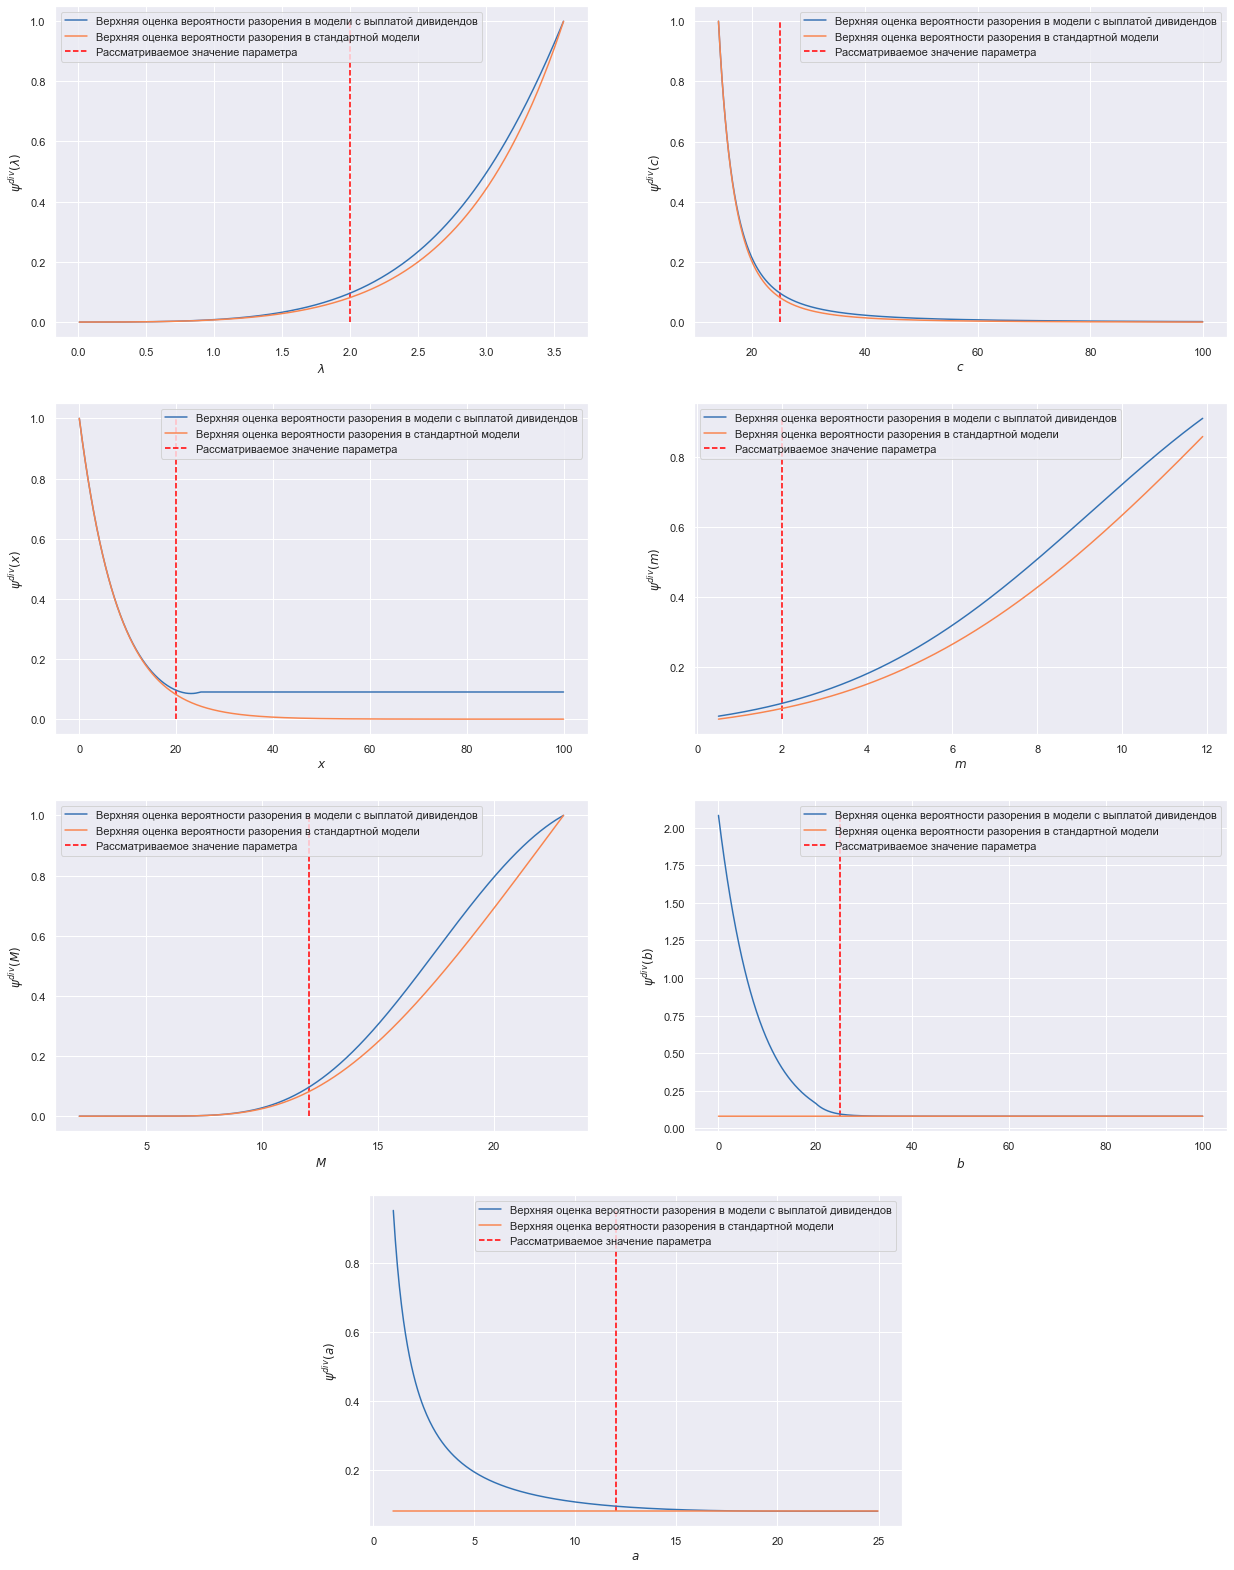
\includegraphics[scale=0.4]{images/params_relation_1.png}
\captionsetup{justification=centering}
\caption{Зависимость теоретических оценок вероятностей разорения от каждого из параметров $\lambda,\ c,\ x,\ m,\ M,\ b,\ a$.}
\label{prob_to_params_relation_1}
\end{figure}

\clearpage

\subsection{Моделирование истории капитала акционерной страховой компании}

Далее мы перешли непосредственно к моделированию с использованием установленных параметров модели. Мы реализовали интерфейсы для линейной барьерной функции и самой модели страховой компании: \texttt{LinearBarrier} и \\
\texttt{KLStockInsuranceModel}. С помощью этих классов получили одну из реализаций случайного процесса, соответствующего капиталу страховой компании, и изобразили ее на графике (рис. \ref{stock_trajectory}).

\begin{figure}[h]
\centering
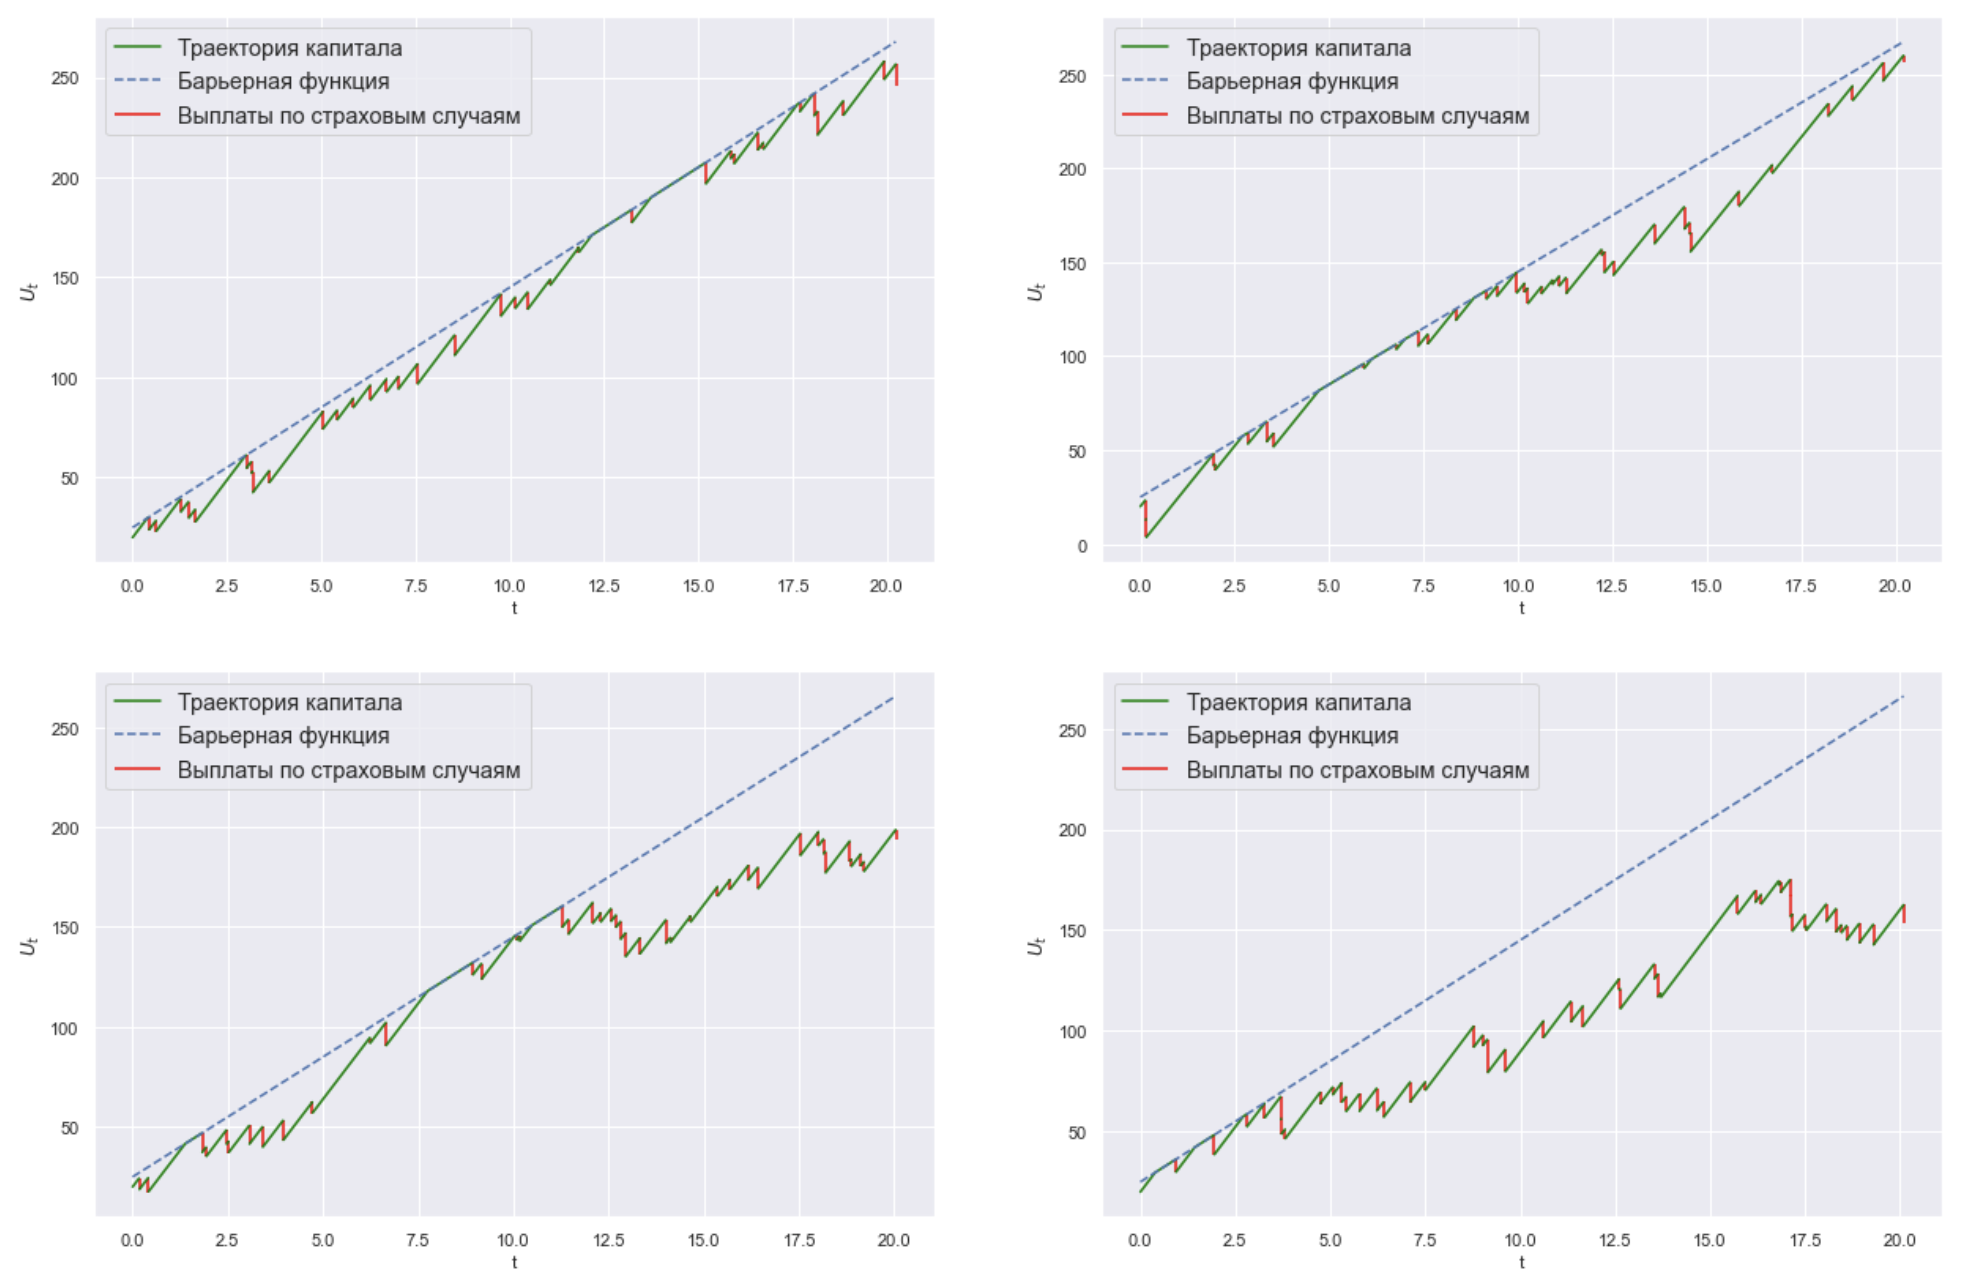
\includegraphics[scale=0.5]{images/KL_stock_trajectory.png}
\captionsetup{justification=centering}
\caption{Траектории капитала акционерной страховой компании с линейной стратегией выплаты дивидендов при $\lambda = 2,\ c = 25,\ x = 20,\ m = 2,\ M = 12,\ b = 25,\ a = 12$.}
\label{stock_trajectory}
\end{figure}
%Желательно показать несколько траекторий и сделать графики более понятными. Плюс добавить параметры, для которых построена модель. Сделайте так, чтобы стр. 7 не была полупустой. Предложение актуально.

По графикам видно, что барьерная функция оказывает небольшое влияние на капитал страховой компании. Скорее всего это связано с установленными параметрами модели: оценка вероятности разорения относительно большая. Соответственно, и значение капитала компании как правило будет лежать ниже барьереной функции.

\subsection{Сравнение оценки вероятности разорения с эвристической оценкой вероятности, полученной с помощью метода Монте-Карло}

После того, как мы получили численное представление оценки вероятности разорения и научились моделировать изменение капитала страховой компании с течением времени, мы смогли приступить к сравнению вычисленной оценки с результатами реального моделирования.

Для получения эмпирической оценки вероятности разорения мы использовали метод Монте-Карло: для разлиных временных огарничений мы 5000 раз запускали моделирование и считали, сколько раз модель приходила к разорению. Таким образом, мы проверяли справедливость утверждения \ref{claim_2} на ограниченном временном отрезке. Результаты первого эксперимента отразили на графике (рис. \ref{MC_1}).

\begin{figure}[h]
\centering
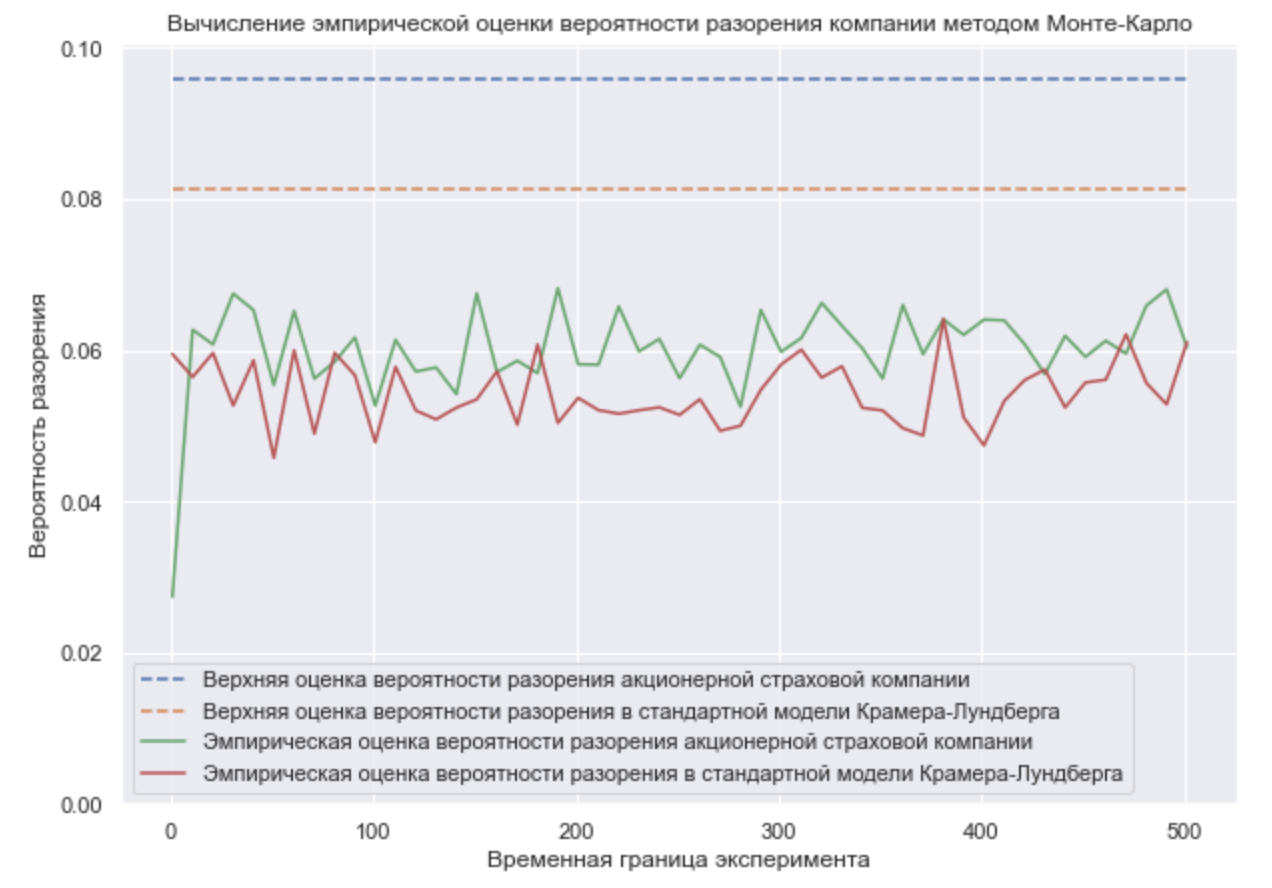
\includegraphics[scale=0.7]{images/KL_stock_MC_1.png}
\captionsetup{justification=centering}
\caption{Сравнение теоретических и эмпирических оценок вероятности разорения, полученных при помощи метода Монте-Карло для стандартной модели Крамера-Лундберга и модели акционерной страховой компании при $\lambda = 2,\ c = 25,\ x = 20,\ m = 2,\ M = 12,\ b = 25,\ a = 12$.}
\label{MC_1}
\end{figure}
%Параметры всех моделей указать и объяснить, из каких соображений их выбираете. Возможно, построить зависимость вероятности разорения от параметров модели.

Из графика видно, что вероятность разорения акционерной страховой компании как правило выше -- это ожидаемый результат, ведь выплата дивидендов негативно влияет на размер капитала компании. Вместе с этим ни одна из эмпирических оценок не превосходит своей верхней теоретической оценки. Тем не менее, оценка вероятности разорения для модели с выплатой дивидендов кажется избыточной, ведь даже значение стандартной оценки вероятности лежит выше графика эмпирической оценки. Мы предположили, что это может быть также связано с неудачным выбором параметров модели: чем менее благоприятными они являются, тем более модели с выплатой дивидендов и без выплаты дивидендов становятся друг на друга похожи. Поэтому при выборе более благоприятных параметров модели разница может быть существеннее. Это также подтверждается графиками на рис. \ref{prob_to_params_relation_1}: отличия в теоретических оценках при заданных параметрах несущественны.

Чтобы получить более наглядную картину, мы изменили параметры модели и повторили эксперимент (рис. \ref{MC_2}) для $\lambda = 2,\ c = 35,\ x = 15,\ m = 2,\ M = 12,\ b = 18,\ a = 7$. По рис. \ref{prob_to_params_relation_1} видно, что наибольшие отличия в моделях наблюдаются при меньших значениях $a$ и $b$ -- именно эти параметры барьерной функции мы поменяли в первую очередь. В действительности, мы также изменили параметры $x$ и $c$, отвечающие за начальный капитал и поступления средств в него соответственно, -- это было сделано для того, чтобы выполнялось начальное условие $x < b$, а также для того, чтобы скорректировать увеличение вероятности разорения за счет ускорения поступления средств в капитал.

\begin{figure}[h]
\centering
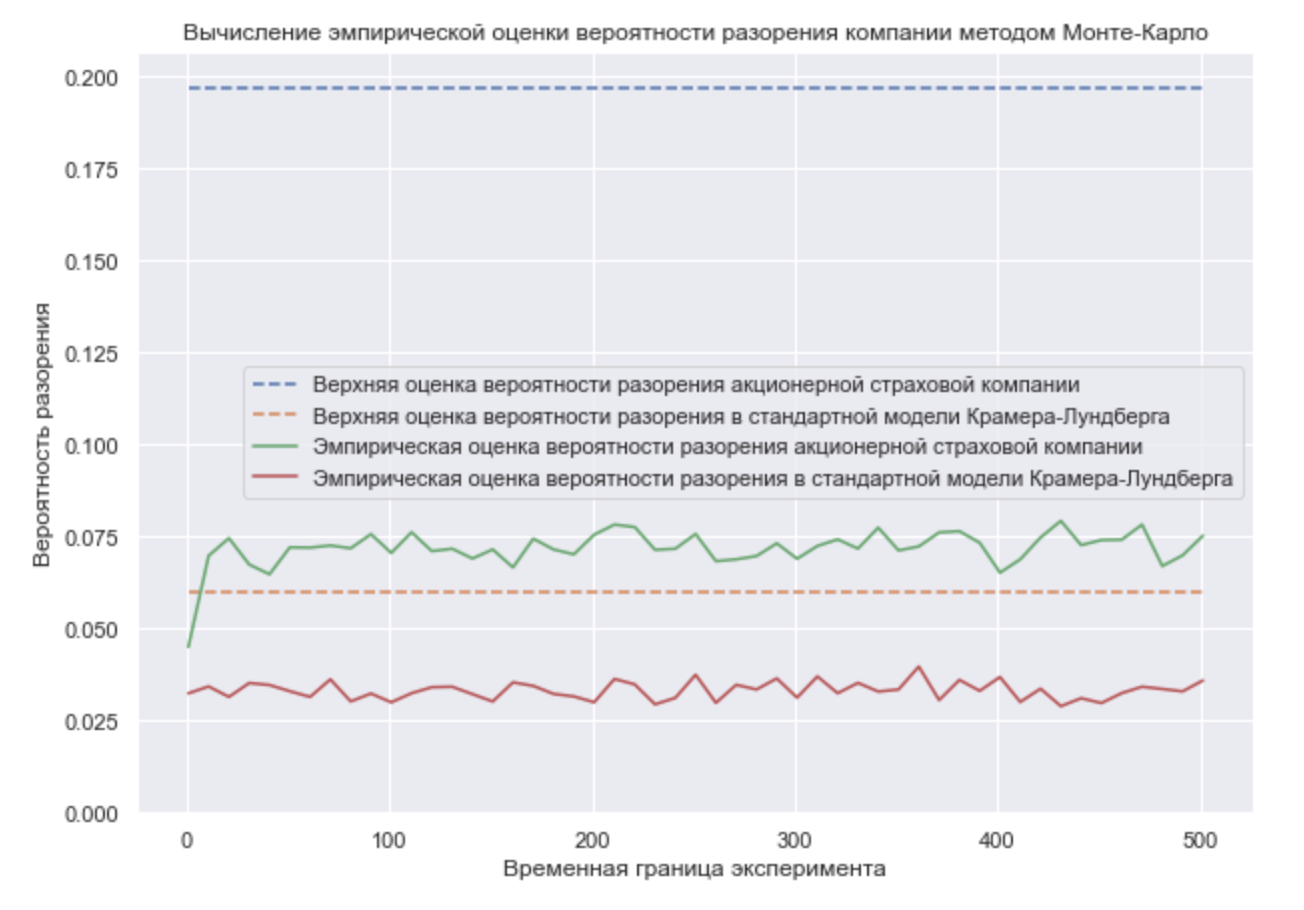
\includegraphics[scale=0.7]{images/KL_stock_MC_2.png}
\captionsetup{justification=centering}
\caption{Сравнение теоретических и эмпирических оценок вероятности разорения, полученных при помощи метода Монте-Карло для стандартной модели Крамера-Лундберга и модели акционерной страховой компании с альтернативными параметрами $\lambda = 2,\ c = 35,\ x = 15,\ m = 2,\ M = 12,\ b = 18,\ a = 7$.}
\label{MC_2}
\end{figure}

График существенно изменился. Эмпирическая оценка вероятности разорения теперь лежит между двумя теоретическими оценками. Это означает, что оценка вероятности разорения стандартной модели Крамера-Лундберга для модели акционерной компании не работает, а наша полученная оценка является правильной.

\subsection{Эксперименты с нелинейной барьерной функцией}

В заключительном этапе практической работы мы решили убедиться, что построенная модель может работать и с другой барьерной функцией, отличной от линейной. В качестве примера мы взяли функцию вида $b_t = b + a \sqrt[4]{t}$. На следующих графиках (рис. \ref{nonlinear_stock_trajectory}, \ref{nonlinear_MC}) изображены соответственно история изменения капитала страховой компании при единичном запуске моделирования и график эмпирической оценки вероятности разорения в зависимости от временного ограничения, полученный по аналогичному методу Монте-Карло.

\begin{figure}[h]
\centering
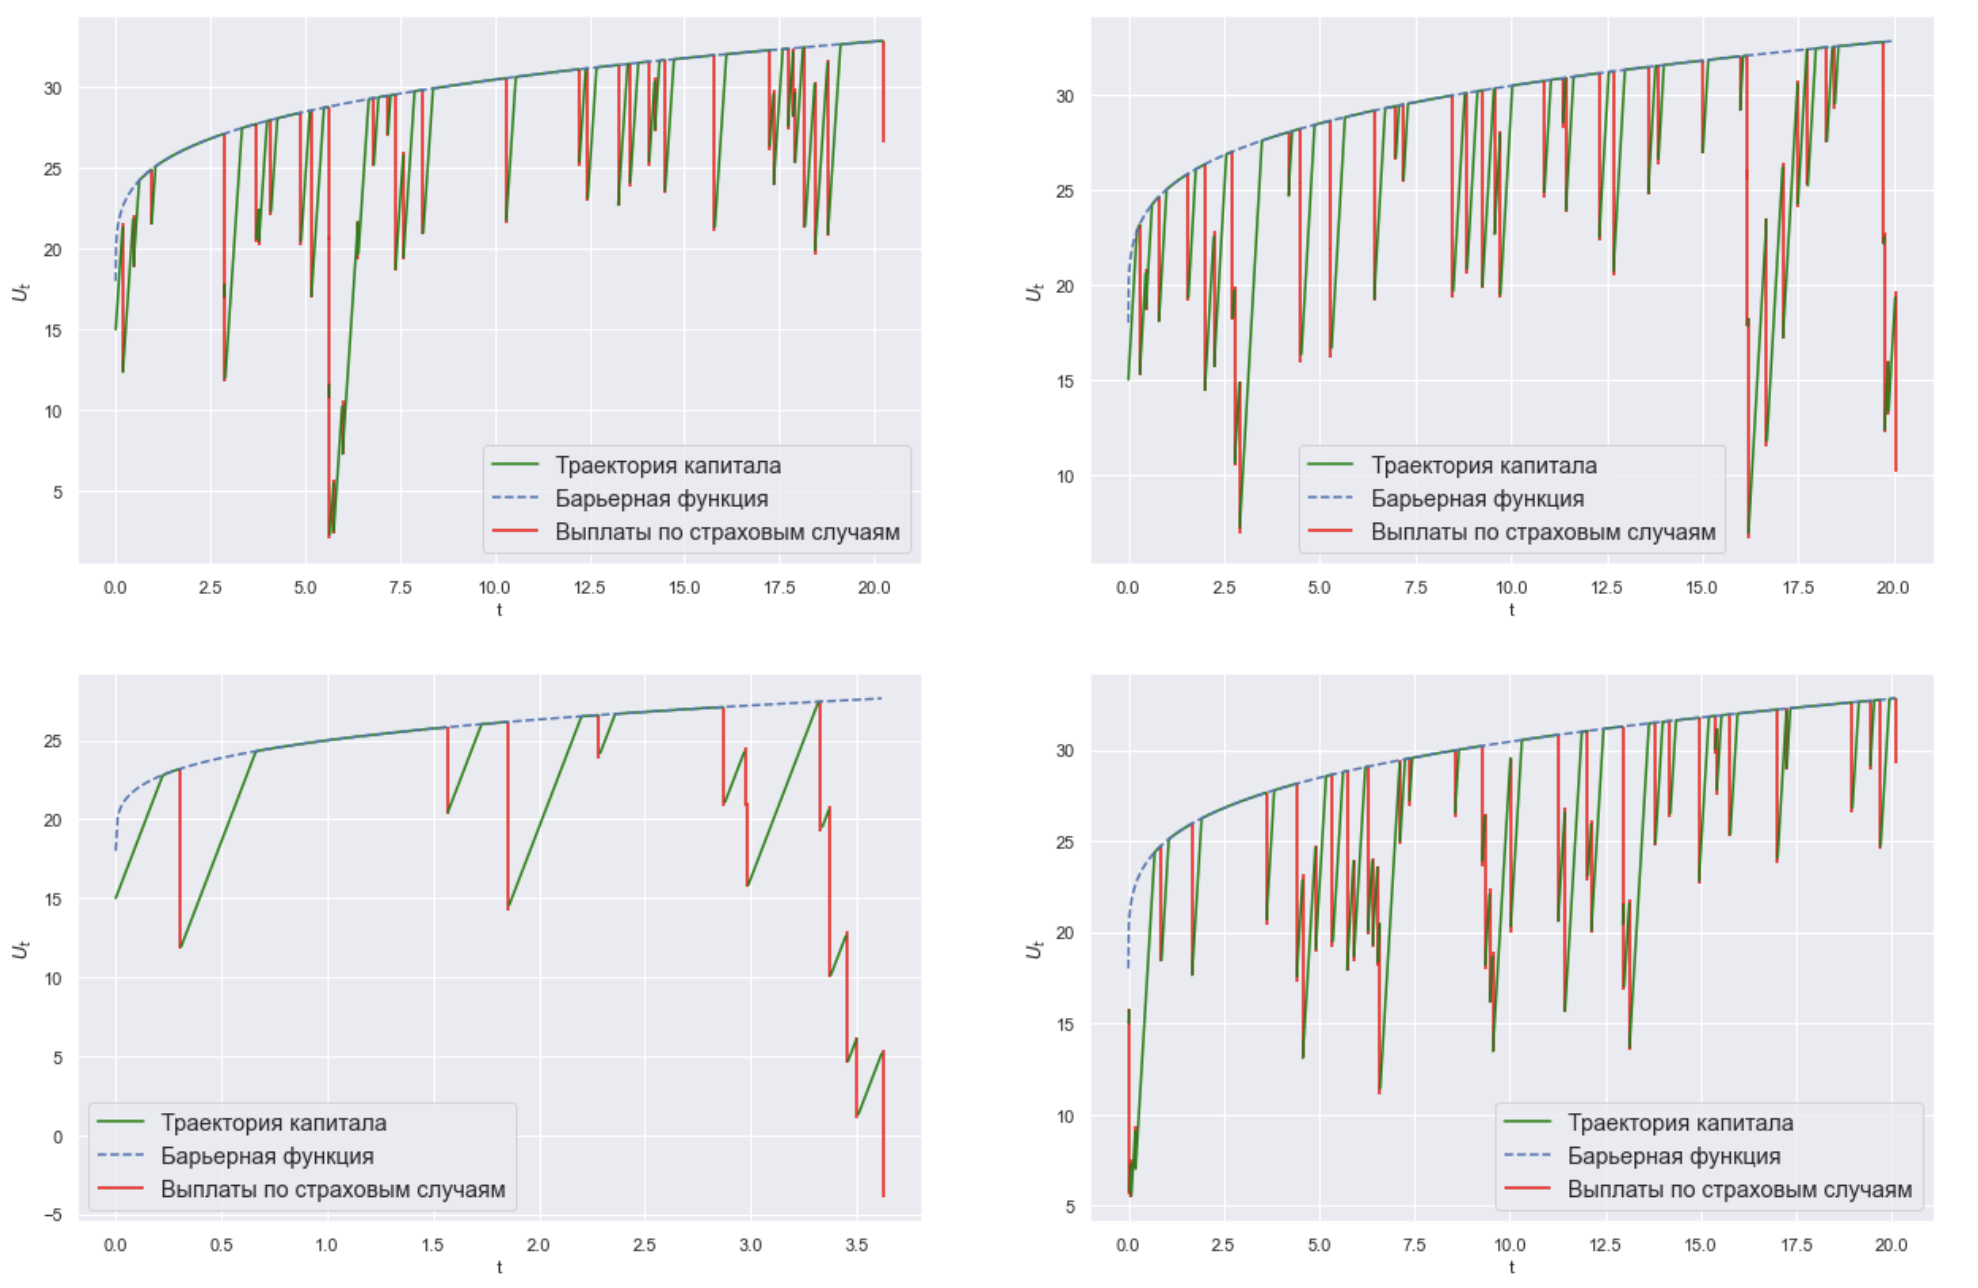
\includegraphics[scale=0.5]{images/nonlinear_barrier_trajectory.png}
\captionsetup{justification=centering}
\caption{Траектории капитала акционерной страховой компании с нелинейной стратегией выплаты дивидендов.}
\label{nonlinear_stock_trajectory}
\end{figure}

\begin{figure}[h]
\centering
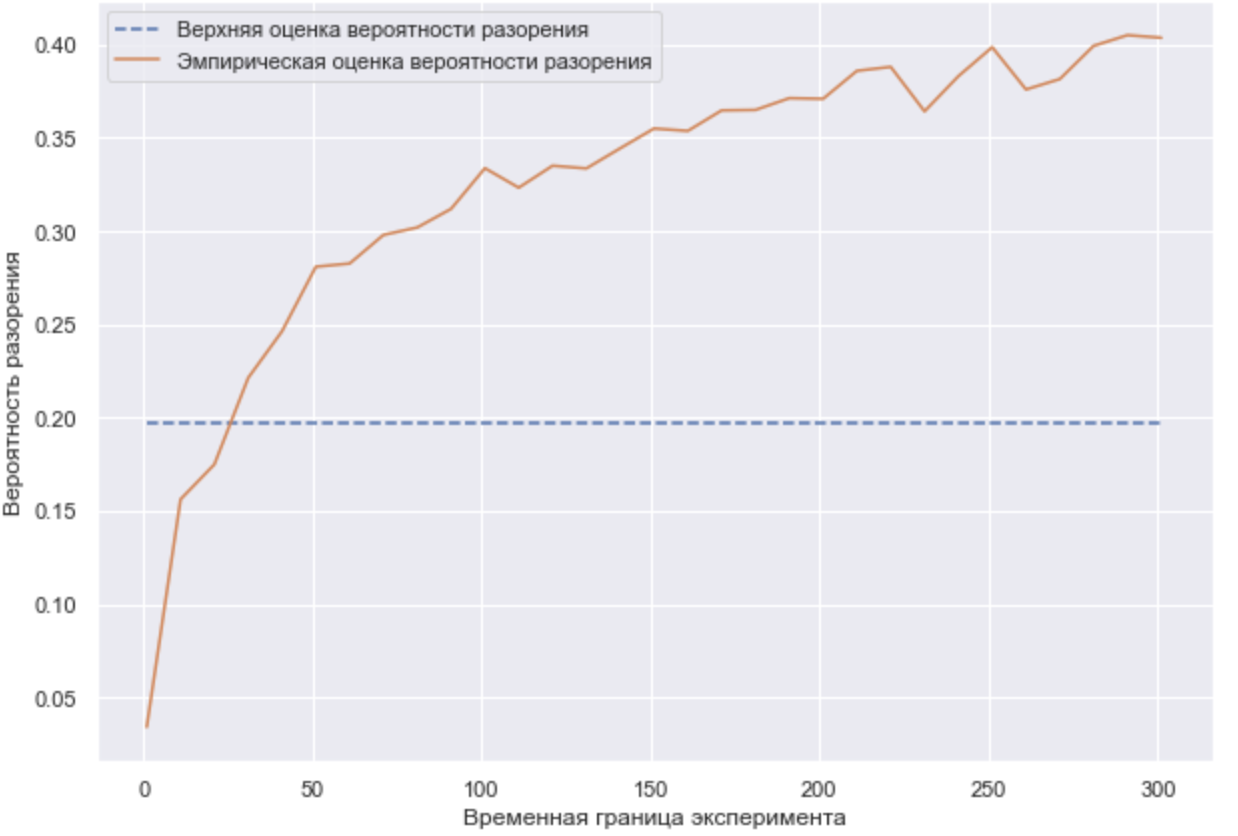
\includegraphics[scale=0.6]{images/non_linear_barrier_MC.png}
\captionsetup{justification=centering}
\caption{Сравнение теоретической и эмпирической оценок вероятности разорения, полученных при помощи метода Монте-Карло для модели акционерной страховой компании нелинейной стратегией выплаты дивидендов.}
\label{nonlinear_MC}
\end{figure}

На рис. \ref{nonlinear_MC} мы для наглядности оставили уровень верхней оценки для схожей модели с линейной стратегией выплаты дивидендов, чтобы показать, что при сублинейной барьерной функции полученная оценка не справедлива.

\clearpage

\section{Результаты}

В ходе работы над проектом мы углубились в проблему моделирования капитала страховых компаний и получили ряд полезных результатов по этой теме:

\begin{itemize}
    \item рассмотрели различные подходы к описанию моделей страховых компаний, мы изучили работы по следующим темам: стандартные модели Крамера-Лундберга и Спарре-Андерсена, модель Крамера-Лундберга со стохастическими премиями, а также модель акционерной страховой компании в рамках модели Спарре-Андерсена;
    
    \item реализовали нахождение верхней оценки вероятности разорения акционерной страховой компании в рамках модели Крамера-Лундберга с линейной стратегией выплаты дивидендов;
    
    \item создали интерфейсы для стандартной и акционерной моделей страховых компаний с возможностью задания произвольной барьерной стратегии выплаты дивидендов;
    
    \item провели моделирование траекторий капитала акционерной страховой компании;
    
    \item нашли эмпирические оценки вероятностей разорения на ограниченном временном интервале с применением метода Монте-Карло.
\end{itemize}

% Постарайтесь выводы указать понятно и тезисно, чтобы было видно, в чем Ваше исследование и в чем Ваш результат.

\section{Выводы}

После проведения экспериментов мы убедились, что их результаты соответствуют теоретическим выкладкам: эмпирические оценки вероятности разорения не превосходят своих верхних оценок. Мы также показали, что выплаты дивидендов могут существенно влиять на вероятность разорения компании -- при определенных параметрах модели ее эмпирическая оценка превосходит верхнюю оценку вероятности разорения в стандартной модели Крамера-Лундберга с теми же параметрами без выплаты дивидендов.

В конце концов, мы убедились, что наша реализация модели акционерной страховой компании может работать с различными барьерными функциями, и показали, что для сублинейных барьерных функций полученная оценка может не выполняться.

Результаты данной работы могут быть полезны для прогнозирования работы страховой компании, а также для подбора подходящей стратегии выплат дивидендов и получения нужного уровня вероятности разорения. Программный код проекта способен предоставить удобный интерфейс для получения наглядных графиков с возможными траекториями капитала компании и может быть использован для будущих исследований.

При инвестировании или учреждении страховой компании важно оценивать возможные риски, и данная работа может стать отправной точкой для дальнейшего прогнозирования.

\clearpage

\bibliographystyle{unsrt}
\bibliography{refs.bib}

\end{document}
